\documentclass{beamer}
\usetheme[block=fill]{metropolis}

\usepackage[english]{babel}
%\usepackage[utf8]{inputenc}

% For notes
\usepackage{pgfpages}
\setbeameroption{show notes on second screen=right}
\usepackage{appendixnumberbeamer} % don't number the backup slides

\usepackage{amsmath,amssymb} % math
\usepackage{graphicx} % images
\DeclareGraphicsExtensions{.eps,.pdf,.png,.jpg,.gif}
\graphicspath{{./img/}}
\usepackage[export]{adjustbox}

\title{aursec - A blockchain approach to securing software packages}
\author{Lukas Krismer \& Bennett Piater}
\institute{Universität Innsbruck - QE - Christian Sillaber}
\date{\today}

\begin{document}

\maketitle


\begin{frame}
	\frametitle{Outline}
	\tableofcontents
	\note{1 min L | }
	%ich werde nie auf die Notes schauen (nur zum Üben) - L
	\note{Liebe Anwesende,
		Mein Name ist Lukas, und Bennett und ich werden euch heute unser Bachelorarbeitsthema näherbringen. Da oben steht so eine schöne große Überschrift ...

	    Aursec - A blockchain approach to securing software packages

		Und wir möchten heute ein bisschen darauf eingehen wie man Softwarepakete, in unserem Fall von der AUR, sicherer machen kann.
		Am Anfang werden wir auf die AUR und ihre Probleme eingehen und später zeigen wir dann, wie wir Teilprobleme mithilfe einer Blockchain lösen wollen. Zum Schluss schauen wir dann noch unser Zeitmanagement und unsere Verantwortlichkeitsverteilung an.}
\end{frame}

\section{AUR}

\begin{frame}{AUR}
	\begin{itemize}
		\item \textbf{AUR}=\alert{A}rch Linux \alert{U}ser \alert{R}epository
		\item Contains package build scripts (PKGBUILDs)
		\item Packages can be voted for inclusion in the official repositories
		\item Easy to use using so-called AUR helpers
		\item Everybody can upload PKGBUILDs
		\item Anyone can adopt orphaned packages
	\end{itemize}
	\note{2min L | }
	\note{Kommen wir zur AUR, also der Arch Linux User Repo. Sie ist eine inoffizielle Repo von Arch Nutzern für Arch Nutzer. Sie beinhaltet Skripte (sog. PKGBUILDs) die für die Erstellung von Paketen benötigt werde . Weiters kann man für Pakete abstimmen um damit eine Aufnahme in die offizielle Community Repo zu fördern. Durch die AUR-helper ist die AUR sehr einfach zu bedienen. So sind yaourt, aurutils und co sehr ähnlich zu bedienen wie Packetmanager. Ein wichtiger Punkt der AUR ist weiters, dass jeder PKGBUILDs hochladen kann. Dies ist sowohl ein sehr großer Vorteil, da es dadurch für fast jedes Problem ein passendes Paket in der AUR gibt,  als auch Nachteil, da die PKGBUILDs fast ausschließlich von Ihren Nutzern validiert werden. So können sich bei unbekannten PKGBUILDs sehr leicht schwarze Schafe einschleichen, die Schadecode enthalten. Der letzte wichte Punkt ist, dass nichtverwaltete Pakete von jedem übernommen werden können, dies wiederum ist ein zweischneidiges Schwert, da dadurch auch böswillige Nutzer Zugriff erhalten können.}
\end{frame}

\begin{frame}[t]{Threat Assessment}
	\begin{columns}
		\column{\dimexpr\paperwidth}
		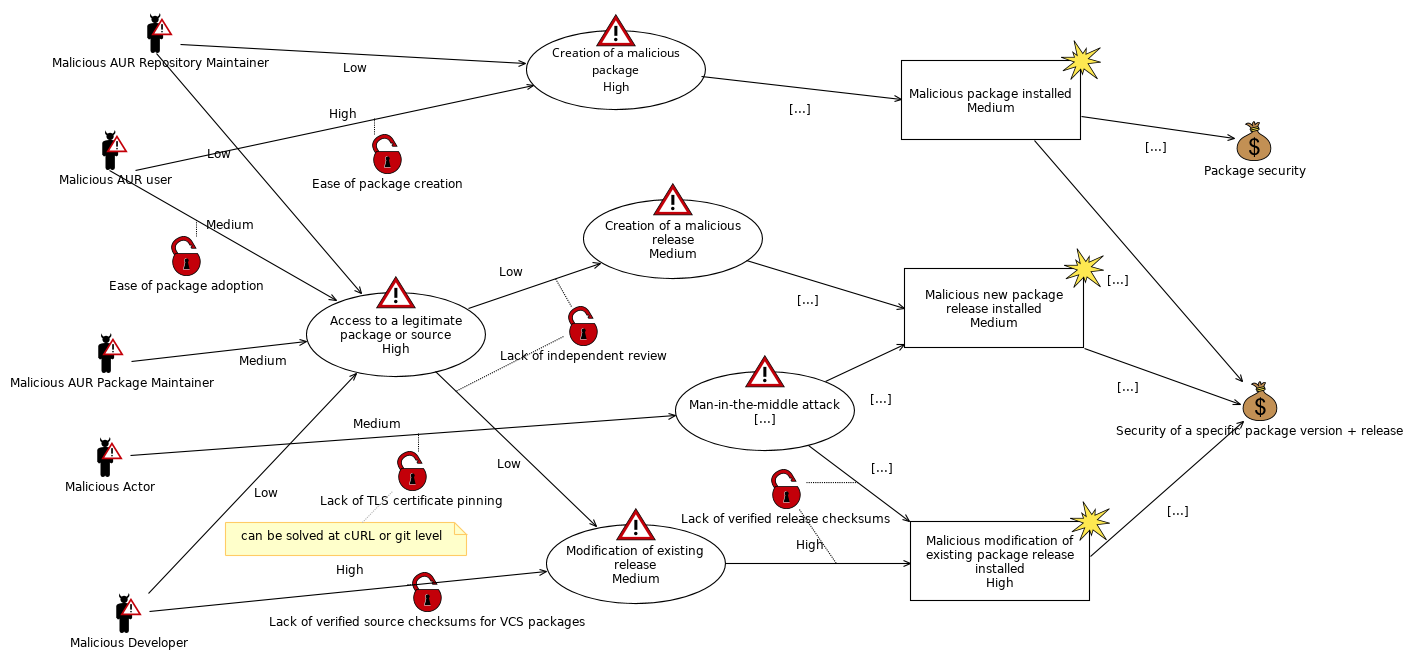
\includegraphics[width=\paperwidth,height=0.7\paperheight,left]{threat.png}
	\end{columns}
	\note{2 min B | Besonderes Augenmerk auf:

	\begin{itemize}
		\item Die grundlegenden Probleme der AUR sind praktisch unlösbar
		\item Zu viele haben Zugang zu Quellen und/oder Buildskripten
		\item Daher: Server-Seitige Signaturen würden nur MITM verhindern
		\item Bösartige Pakete, Releases oder Veränderungen sehr einfach
	\end{itemize}}
\end{frame}

\section{Our Project}

\begin{frame}{Covered Threats}
	\begin{columns}
		\column{\dimexpr\paperwidth}
		\includegraphics<1>[width=\paperwidth,height=0.7\paperheight,left]{threat.png}
		\includegraphics<2>[width=\paperwidth,height=0.7\paperheight,left]{threat2.png}
	\end{columns}
	\note{1 min L | }
	\note{ Kommen wir zu unserem Projekt. Wenn wir uns wieder unsere Threatanalyse anschauen, sehen wir hier "zeig" , dass die validierung der Version große Probleme beheben könnte. Und genau dies wollen wir tun. Mithilfe einer Blockchain sollte es uns Möglich sein dieses Problem zu beseitigen und somit auch die Urprobleme, wie Modifikationen eines Releases oder ein teil des man-in-the-middle Agriffs zu beheben}
	\end{frame}

	\begin{frame}{Basic Workflow of the Core Library}
	\begin{center}
	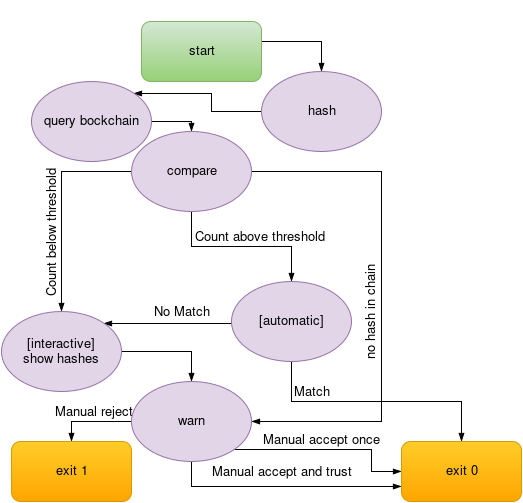
\includegraphics[height=0.9\textheight]{workflow.png}
	\end{center}
	\note{3 min L | }
	\note{0) herunterladen des PKGBUILDs des gewollten Paketes
		0) Wir generieren lokal einen Hash des PKGBUILDs des Paketes
		2) Wir fragen für das Paket den Hash aus der Blockchain ab
		3) Wir bekommen die Anzahl des Hashes + Hash für dieses Paket
		4) 3 Möglichkeiten
			1) kein Hash vorhanden
				Warnung Manuelles akzeptieren oder ablehnen
			2) unterhalb des Treshold. Der Treshold ist eine Grenze bei der unser Programm automatisch den Hash als aussagekräftig und glaubhaft sieht.
				beide Hashes werden angezeigt
				Manuelles akzeptieren oder ablehnen
			3) über dem Treshold
				1) falsche Hash
					beide Hashes werden angezeigt
					Manuelles akzeptieren oder ablehnen
				2) richtiger Hash (gewollte Fall)
					automatisches akzepieren --> automatisch in die Blockchain schreiben

		2 Möglichkeiten vom manuellen akzeptieren, glaubwürdigkeit des Hashes}
\end{frame}

\begin{frame}{Components}
	\begin{itemize}
		\item Program on a private Ethereum blockchain
		\item Shell library
		\item AUR package
		\item Integration in aurutils
		\item Threat analysis of the AUR and our software
		\item Web- and/or CLI-Interface for stats/events
	\end{itemize}
	\note{2 min B

	\begin{itemize}
		\item Das eigentliche Programm zum Speichern der Hashes
		\item Unsere Library, die den Workflow automatisiert
		\item Ein Paket für die AUR
		\item Integration in einen der Besten AUR-Helper \\
		--> Im Zuge dessen allgemein nützliche Beiträge dazu
	    \item Threat-analysen, um die Gefährdungsstufe und die Qualität unseres Beitrags einzuschätzen
	    \item Ein Interface, mit dem die Aktivität der Blockchain überwacht werden kann
	\end{itemize}}
\end{frame}

\begin{frame}{Schedule}
	\begin{itemize}
		\item \textbf{25.10} \emph{prototype:} hashing \hfill B
		\item \textbf{08.11} \alert{Initial Presentation}\hfill L
		\item \textbf{15.11} \emph{prototype:} library without blockchain back-end \hfill B/L
		\item \textbf{15.11} Bash-API for the blockchain \hfill L
		\item \textbf{30.11} \emph{finish:} \alert{Solidity program} \hfill B
		\item \textbf{08.12} deploy local blockchain for development \hfill L
		\item \textbf{08.12} running server with ethereum-node \hfill B/L
		\item \textbf{15.12} \emph{prototype:} \alert{Library} incl. back-end \hfill L
		\item \textbf{20.12} \emph{contrib:} pre-build-hooks in aurutils \hfill B
	\end{itemize}
	\note{2 min B

	Wir haben eine sehr \textbf{detaillierte Planung} ausgearbeitet.
	Einerseits benötigen wir sie, um effizient \textbf{kooperieren} zu können und zügig voran zu kommen; Andererseits soll sie uns auch ein Maximaltempo vergeben, denn wir tendieren beide eher dazu, uns zu \textbf{überarbeiten}.

	\begin{itemize}
		\item Solidity-program auf Blockchain
		\item Library-Prototyp
		\item Beiträge zum AUR-Helper aurutils über Weihnachten
	\end{itemize}
	}
\end{frame}

\begin{frame}{Schedule}
	\begin{itemize}
		\item \textbf{10.01} \emph{contrib:} TLS-public-key-pinning in aurutils \hfill B
		\item \textbf{10.01} configuration and trust-cutoff \hfill L
		\item \textbf{15.01} \emph{test:} \alert{Integration in aurutils} \hfill B
		\item \textbf{15.02} \alert{AUR package} incl. private blockchain \hfill B
		\item \textbf{01.03} \emph{finish:} libary and aurutils-Hook \hfill B
		\item \textbf{31.03} \emph{finish:} Web- and/or CLI-Interface \hfill L
		\item \textbf{21.04} \alert{Draft paper} for feedback\hfill
		\item \textbf{??.05} \emph{finish:} Paper\hfill
		\item \textbf{??.05} Final presentation\hfill L
	\end{itemize}
	\note{2 min B

	\begin{itemize}
		\item am 15.01 mit aurutils testbar
		\item AUR-Paket zur einfachen Verbreitung
		\item Programmierung endet am 31. März
		\item Meiste Schreibarbeit im April und besonders über Ostern
		\item Abgabe bequem for den Klausuren
	\end{itemize}}
\end{frame}

\begin{frame}[standout]
	Questions?
\end{frame}


\end{document}
